% Real-data per-batch latency scaling — (1,1.819) (20,4.386) (40,6.016) (60,6.183) (80,6.263) (100,7.920) (120,7.719) (140,7.535) (160,8.748) (180,6.702) (200,7.162) (220,8.248) (240,7.399) (260,6.536) (280,7.283) (300,7.579) (320,8.517) (340,6.851) (360,7.099) (380,6.883) (400,8.989) (420,8.732) (440,8.274) (460,8.101) (480,8.169) (500,8.931) (520,8.727) (540,8.918) (560,8.608) (580,9.319) (600,7.779) (620,8.303) (640,9.060) (660,8.185) (680,8.455) (700,9.460) (720,7.622) (740,7.765) (760,9.469) (780,8.693) (800,9.985) (820,9.338) (840,8.268) (860,9.259) (880,9.610) (900,9.187) (920,9.318) (940,8.961) (960,9.561) (980,9.424) (1000,9.040) vs Flink vs Spark (51 pts, step-20, full 3.6 GB).
% Double-column standalone; pdflatex + pgfplots. Data: NES+Flink from nes_vs_flink_vs_spark_scaling_step20
% (run_group 20260817T164347-3ec56b98); Spark = REAL per-batch (64 MiB file-microbatch-csv source) from
% nes_vs_flink_vs_spark_scaling_step20_spark_mb (run_group 20260820T144859-a82252ff, 2026-08-21).
\documentclass[tikz,border=6pt]{standalone}
\usepackage{pgfplots}
\pgfplotsset{compat=1.16}
\definecolor{nescol}{HTML}{2CA02C}
\definecolor{flinkcol}{HTML}{7D5BBE}
\definecolor{sparkcol}{HTML}{E69F00}
\begin{document}
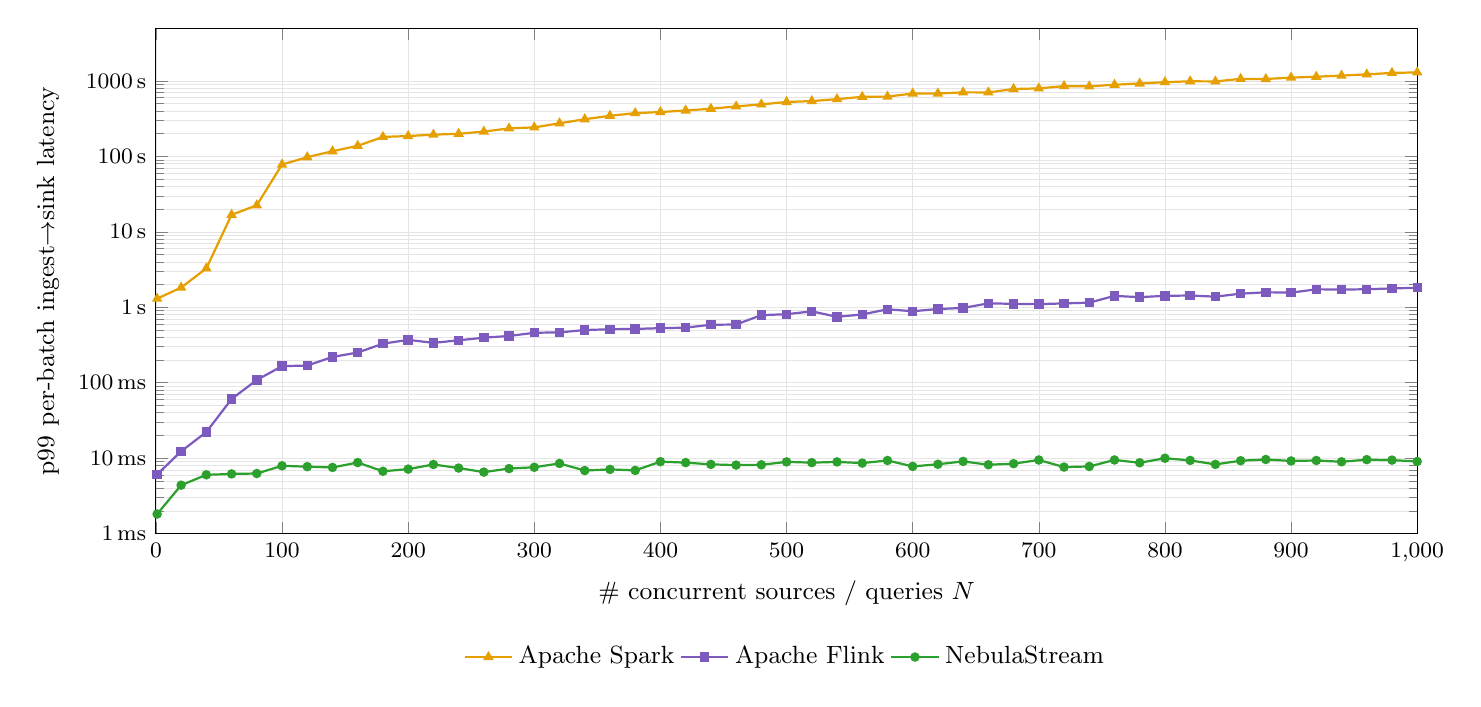
\begin{tikzpicture}
\begin{axis}[
  width=17.6cm, height=8.0cm,
  ymode=log, ymin=1, ymax=5e6,
  xmin=0, xmax=1000, xtick={0,100,200,300,400,500,600,700,800,900,1000},
  ytick={1e0,1e1,1e2,1e3,1e4,1e5,1e6},
  yticklabels={1\,ms,10\,ms,100\,ms,1\,s,10\,s,100\,s,1000\,s},
  xlabel={\# concurrent sources / queries $N$},
  ylabel={p99 per-batch ingest$\to$sink latency},
  label style={font=\small}, tick label style={font=\footnotesize},
  grid=both, grid style={gray!20, very thin},
  legend style={font=\small, at={(0.5,-0.20)}, anchor=north, legend columns=3, draw=none},
  legend cell align=left, every axis plot/.append style={mark options={solid}},
]
\addplot[sparkcol, thick, mark=triangle*, mark size=1.4pt] coordinates {(1,1302.000) (20,1826.000) (40,3279.000) (60,16826.000) (80,22511.000) (100,78060.000) (120,97545.000) (140,117095.000) (160,138142.000) (180,181273.000) (200,186064.000) (220,194319.000) (240,199441.000) (260,213262.000) (280,235073.000) (300,242472.000) (320,274600.000) (340,310971.000) (360,345476.000) (380,374420.000) (400,387126.000) (420,405897.000) (440,428292.000) (460,459937.000) (480,489476.000) (500,525893.000) (520,541133.000) (540,574246.000) (560,615256.000) (580,620805.000) (600,680611.000) (620,681879.000) (640,706184.000) (660,704602.000) (680,782739.000) (700,796558.000) (720,854378.000) (740,847814.000) (760,891221.000) (780,925251.000) (800,962888.000) (820,989556.000) (840,985543.000) (860,1066125.000) (880,1061625.000) (900,1108391.000) (920,1137107.000) (940,1178119.000) (960,1222122.000) (980,1278620.000) (1000,1297848.000)};
\addlegendentry{Apache Spark}
\addplot[flinkcol, thick, mark=square*, mark size=1.3pt] coordinates {(1,6.093) (20,12.326) (40,22.203) (60,60.795) (80,108.813) (100,165.829) (120,169.007) (140,219.568) (160,251.451) (180,329.051) (200,370.292) (220,337.565) (240,365.073) (260,395.447) (280,416.533) (300,459.275) (320,465.017) (340,499.130) (360,512.009) (380,516.722) (400,528.622) (420,537.138) (440,586.883) (460,590.914) (480,787.034) (500,809.546) (520,882.985) (540,747.870) (560,803.162) (580,940.148) (600,886.493) (620,948.020) (640,980.648) (660,1126.602) (680,1111.817) (700,1100.204) (720,1126.459) (740,1152.242) (760,1415.969) (780,1361.919) (800,1419.439) (820,1432.023) (840,1383.279) (860,1514.391) (880,1580.746) (900,1564.201) (920,1731.084) (940,1716.610) (960,1734.542) (980,1777.562) (1000,1815.114)};
\addlegendentry{Apache Flink}
\addplot[nescol, thick, mark=*, mark size=1.3pt] coordinates {(1,1.819) (20,4.386) (40,6.016) (60,6.183) (80,6.263) (100,7.920) (120,7.719) (140,7.535) (160,8.748) (180,6.702) (200,7.162) (220,8.248) (240,7.399) (260,6.536) (280,7.283) (300,7.579) (320,8.517) (340,6.851) (360,7.099) (380,6.883) (400,8.989) (420,8.732) (440,8.274) (460,8.101) (480,8.169) (500,8.931) (520,8.727) (540,8.918) (560,8.608) (580,9.319) (600,7.779) (620,8.303) (640,9.060) (660,8.185) (680,8.455) (700,9.460) (720,7.622) (740,7.765) (760,9.469) (780,8.693) (800,9.985) (820,9.338) (840,8.268) (860,9.259) (880,9.610) (900,9.187) (920,9.318) (940,8.961) (960,9.561) (980,9.424) (1000,9.040)};
\addlegendentry{NebulaStream}
\end{axis}
\end{tikzpicture}
\end{document}
